\documentclass[../main.tex]{subfiles}
\begin{document}

\chapter{Ordnungsgraphen}
\label{chapter:ordnungsgraphen}

Ein weiteres Beispiel für perfekte Graphen sind Vergleichbarkeitsgraphen. Dies sind jene Graphen $(V, E)$, welche die Vergleichbarkeitsrelation zu einer (strikten) Halbordnung $(V, <)$ darstellen, i.e. $uv \in E \Leftrightarrow u < v \vee v < u$. Ihre Perfektheit ist verglichen\footnote{Ba Dum Tss} nicht so trivial wie die vorherigen Beispiele.

Um im Rahmen der Graphentheorie zu bleiben, interpretieren wir diese strikte Halbordnung selbst als gerichteten Graphen.

\begin{definition}[Vergleichbarkeitsgraph]
    Ein (ungerichteter) Graph $(V, E)$ heißt \emph{Vergleichbarkeitsgraph}, wenn es einen gerichteten Graphen $(V, F)$ gibt, für den gilt:
    \begin{itemize}
        \item Richtungszuweisung: $\forall u, v \in V : uv \in F \vee vu \in F \Leftrightarrow uv \in E$
        \item Transitivität: $\forall u, v, w \in V : uv \in F \wedge vw \in F \Rightarrow uw \in F$
        \item Antisymmetrie: $\forall u, v \in V : uv \in F \Rightarrow vu \notin F$
    \end{itemize}
    Wir nennen den Graphen $(V, F)$ eine \emph{Orientierung} von $(V, E)$.
\end{definition}

Offensichtlich ist Vergleichbarkeitsgraph zu sein ebenfalls eine hereditäre Eigenschaft. Zu gegebener Knotenmenge $A \subset V$ ist $(A, F \cap (A \times A))$ eine Orientierung von $G_A$. Es reicht also wieder nur $\chi(G) = \omega(G)$ im nachfolgenden Teil zu zeigen.

\begin{bemerkung}
    Orientierungen von Vergleichbarkeitsgraphen sind nicht mit Hasse-Diagrammen zu verwechseln. Während in den Orientierungen explizit die Transitivität gefordert wird, sind in Hasse-Diagrammen Kanten, die wegen der Transitivität impliziert werden, weggelassen. (Vgl. Abbildung \ref{fig:hasse})
\end{bemerkung}

\begin{figure}[ht]
    \label{fig:hasse}
    \centering
    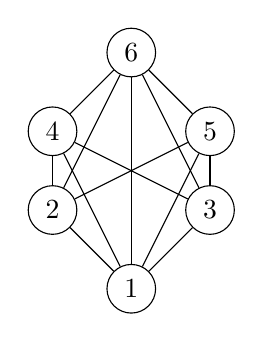
\begin{tikzpicture}
        \node[circle, draw] (u1) at (0, 0) {$1$};
        \node[circle, draw] (u2) at (-1, 1) {$2$};
        \node[circle, draw] (u3) at (1, 1) {$3$};
        \node[circle, draw] (u4) at (-1, 2) {$4$};
        \node[circle, draw] (u5) at (1, 2) {$5$};
        \node[circle, draw] (u6) at (0, 3) {$6$};

        \draw (u1) -- (u2);
        \draw (u1) -- (u3);
        \draw (u1) -- (u4);
        \draw (u1) -- (u5);
        \draw (u1) -- (u6);
        
        \draw (u2) -- (u4);
        \draw (u2) -- (u5);
        \draw (u2) -- (u6);
        
        \draw (u3) -- (u4);
        \draw (u3) -- (u5);
        \draw (u3) -- (u6);

        \draw (u4) -- (u6);
        \draw (u5) -- (u6);
    \end{tikzpicture}
    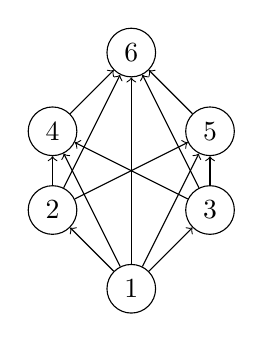
\begin{tikzpicture}
        \node[circle, draw] (u1) at (0, 0) {$1$};
        \node[circle, draw] (u2) at (-1, 1) {$2$};
        \node[circle, draw] (u3) at (1, 1) {$3$};
        \node[circle, draw] (u4) at (-1, 2) {$4$};
        \node[circle, draw] (u5) at (1, 2) {$5$};
        \node[circle, draw] (u6) at (0, 3) {$6$};

        \draw [->] (u1) -> (u2);
        \draw [->] (u1) -> (u3);
        \draw [->] (u1) -> (u4);
        \draw [->] (u1) -> (u5);
        \draw [->] (u1) -> (u6);
        \draw [->] (u2) -> (u4);
        \draw [->] (u2) -> (u5);
        \draw [->] (u2) -> (u6);
        \draw [->] (u3) -> (u4);
        \draw [->] (u3) -> (u5);
        \draw [->] (u3) -> (u6);
        \draw [->] (u4) -> (u6);
        \draw [->] (u5) -> (u6);
    \end{tikzpicture}
    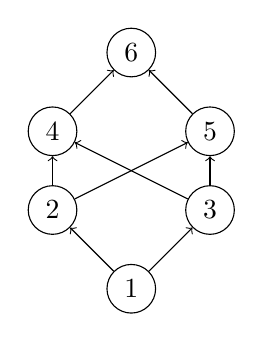
\begin{tikzpicture}
        \node[circle, draw] (u1) at (0, 0) {$1$};
        \node[circle, draw] (u2) at (-1, 1) {$2$};
        \node[circle, draw] (u3) at (1, 1) {$3$};
        \node[circle, draw] (u4) at (-1, 2) {$4$};
        \node[circle, draw] (u5) at (1, 2) {$5$};
        \node[circle, draw] (u6) at (0, 3) {$6$};

        \draw [->] (u1) -> (u2);
        \draw [->] (u1) -> (u3);
        \draw [->] (u2) -> (u4);
        \draw [->] (u2) -> (u5);
        \draw [->] (u3) -> (u4);
        \draw [->] (u3) -> (u5);
        \draw [->] (u4) -> (u6);
        \draw [->] (u5) -> (u6);
    \end{tikzpicture}
    \caption{Ein Vergleichbarkeitsgraph, eine Orientierung davon sowie das Hasse-Diagramm zur Halbordnung der Orientierung.}
\end{figure}

\begin{satz}
    Sei $(V, E)$ ein Vergleichbarkeitsgraph. Dann ist $(V, E)$ perfekt.
\end{satz}
\begin{proof}
    Sei $(V, F)$ eine Orientierung von $(V, E)$. Wir definieren rekursiv eine sogenannte Höhenfunktion $h$ auf den Knoten:
    \begin{align*}
        h : V &\to \N \\
        v &\mapsto \begin{cases}
            0 &v \text{ ist eine Senke}\\
            \max\limits_{wv \in F} h(w) + 1 &\text {sonst}
        \end{cases}
    \end{align*}
    
    Aufgrund der Transitivität und der Antisymmetrie ist der Graph $(V, F)$ zyklenfrei und weil $V$ endlich ist gibt es mindestens eine Senke. Damit ist $h$ wohldefiniert. Definiere $m := \max_{v \in V} h(v)$.

    Für eine Kante $uv \in F$ gilt
    $$h(u) \leq \max\limits_{wv \in F} h(w) = h(v) - 1 < h(v).$$

    Damit ist $h$ also eine zulässige Knotenfärbung für $(V, E)$ mit $m + 1$ vielen Farben.
    
    Zu einem solchen Knoten $v$, bei dem $h(v) = m$ maximal ist, findet man einen Pfad $v =: u_m, \hdots, u_0$ von $v$ zu einer Senke $u_0$ mit $h(u_i) = i\, \forall i \in \N_{\leq m}$, indem man einfach in jedem Schritt einen Zeugen des Maximums in der Definiton von $h$ als nächsten Knoten wählt. Aufgrund der Transitivität von $F$ ist $\{u_i : i \in \N_{\leq m}\}$ sogar eine $m+1$ große Clique.
    
    Es kann also keine größere Clique und keine kleinere Färbung geben und $\chi(G) = m+1 = \omega(G)$. Wegen der Hereditärität ist $(V, E)$ also perfekt.
\end{proof}

\begin{korollar}
    Sei $(V, E)$ ein Vergleichbarkeitsgraph und sei eine Orientierung $(V, E)$ gegeben. Dann kann eine minimale zulässige Färbung $h : V \to \N$, sowie eine maximale Clique in linearer Zeit, also $O(|V| + |F|)$ gefunden werden.
\end{korollar}
\begin{proof}
    
    Die Höhenfunktion $h: V \to \N$ aus dem vorherigen Beweis ist eine zulässige minimale Färbung und kann in linearer Zeit mit Algorithmus \ref{algo:heightfunction} berechnet werden.
    
    \begin{figure}[ht]
        \label{algo:heightfunction}
        \centering
        \begin{minted}{python3}
def compute_height(G: DirectedGraph) -> dict[Vertex, int]:
    h = dict()
    unset_inneighbor_count = {u: u.indegree for u in G.vertices}
    
    def DFS(u: Vertex):
        unset_inneighbor_count[u] -= 1
        if unset_inneighbor_count[u] == 0:
            h[u] = max(h[v] for v in u.in_neighbors) + 1
            for w in u.out_neighbors:
                DFS(w)
        
    for u in G.vertices:
        if u.indegree == 0:
            h[u] = 0
            for v in u.out_neighbors:
                DFS(v)
    
    return h
        \end{minted}
        \caption{Pseudo-Pseudo-Code zur Berechnung der Höhenfunktion. Details zur Implementierung gibt es in Appendix \ref{appendix:code}.}
    \end{figure}
    
    Der Algorithmus läuft über eine Tiefensuche \emph{(eng. Depth-First-Search, DFS)}, wobei $h$ für einen Knoten erst berechnet wird, wenn $h$ für alle Ausgang-Nachbaren bereits berechnet sind. In \verb|unset_outneighbor_count[u]| wird absteigend gezählt, wie oft die Funktion \verb|DFS| für einen Knoten \verb|u| aufgerufen wurde. Sobald \verb|DFS| von jedem seiner Ausgang-Nachbaren aufgerufen wurde und \verb|unset_outneighbor_count[u]| $= 0$ ist sicher, das $h$ für alle Ausgang-Nachbaren von \verb|u| berechnet wurde.
    
    \verb|DFS| wird pro Kante einmal aufgerufen und pro (nicht Senke-)Knoten $u$ wird einmal der Teil innerhalb der \verb|if|-Abfrage ausgeführt, welcher $O(Ausgrad(u))$ für das Maximum und $O(Ingrad(u))$ für das Aufrufen von \verb|DFS| braucht.
    
    Die Vorbereitung von \verb|unset_outneighbor_count| sowie das Durchlaufen der Knoten auf der Suche nach den Senken braucht jeweils $O(|V|)$. Insgesamt braucht der Algorithmus also $O(2\cdot|V| + 3\cdot|F|) = O(|V| + |F|)$ viel Zeit.

    \begin{figure}[ht]
        \label{algo:clique}
        \centering
        \begin{minted}{python3}
def find_path(G: DirectedGraph) -> list[Vertex]:
    h = compute_height(G)

    max_vertex = max(h, key=h.get)
    
    current_vertex = max_vertex
    path = [max_vertex]
    while h[current_vertex] > 0:
        for neighbor in current_vertex.in_neighbors:
            if h[neighbor] == h[current_vertex] - 1:
                current_vertex = neighbor
                break
        path.append(current_vertex)

    path.reverse()
    return path
        \end{minted}
        \caption{Pseudo-Pseudo-Code zur Berechnung einer Clique.}
    \end{figure}

\end{proof}
    
\begin{figure}[ht]
    \label{fig:comparability_graph}
    \centering
    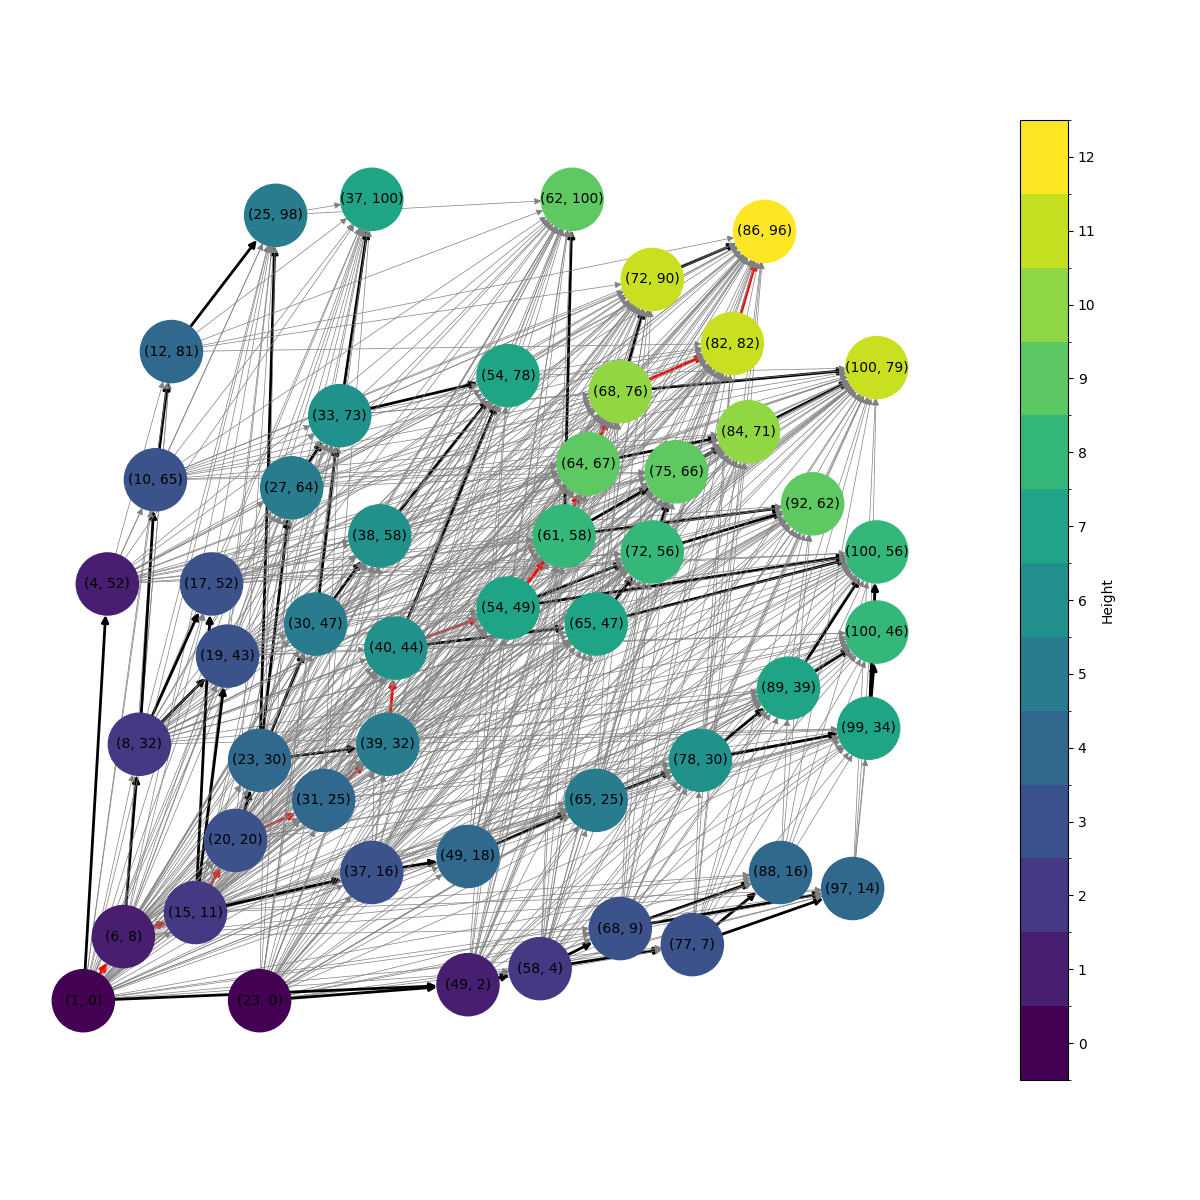
\includegraphics[width=\textwidth]{figures/comparability_graph.png}
    \caption{Beispiel für (die Orientierung eines) Vergleichbarkeitsgraphen. Die Knoten sind Zahlenpaare und $(a, b) < (c, d) :\Leftrightarrow a < c \wedge b < d$. Die Farbe der Knoten entspricht der Höhe $h$. Die dick eingezeichneten Kanten sind jene, wo der Höhenunterschied nur 1 ist. In Rot ist ein maximaler Pfad (und damit eine maximale Clique) eingezeichnet.}
\end{figure}
    


\end{document}